\section{Gegen\"uberstellung aller Simulationen und Messergebnisse}
\label{sec:simmesskomplett}
Im folgenden Abschnitt sind die Gegen\"uberstellungen der Messungen und Simulationen f\"ur alle variablen Parameter zu sehen.

\begin{figure}[htb]
	\centering
	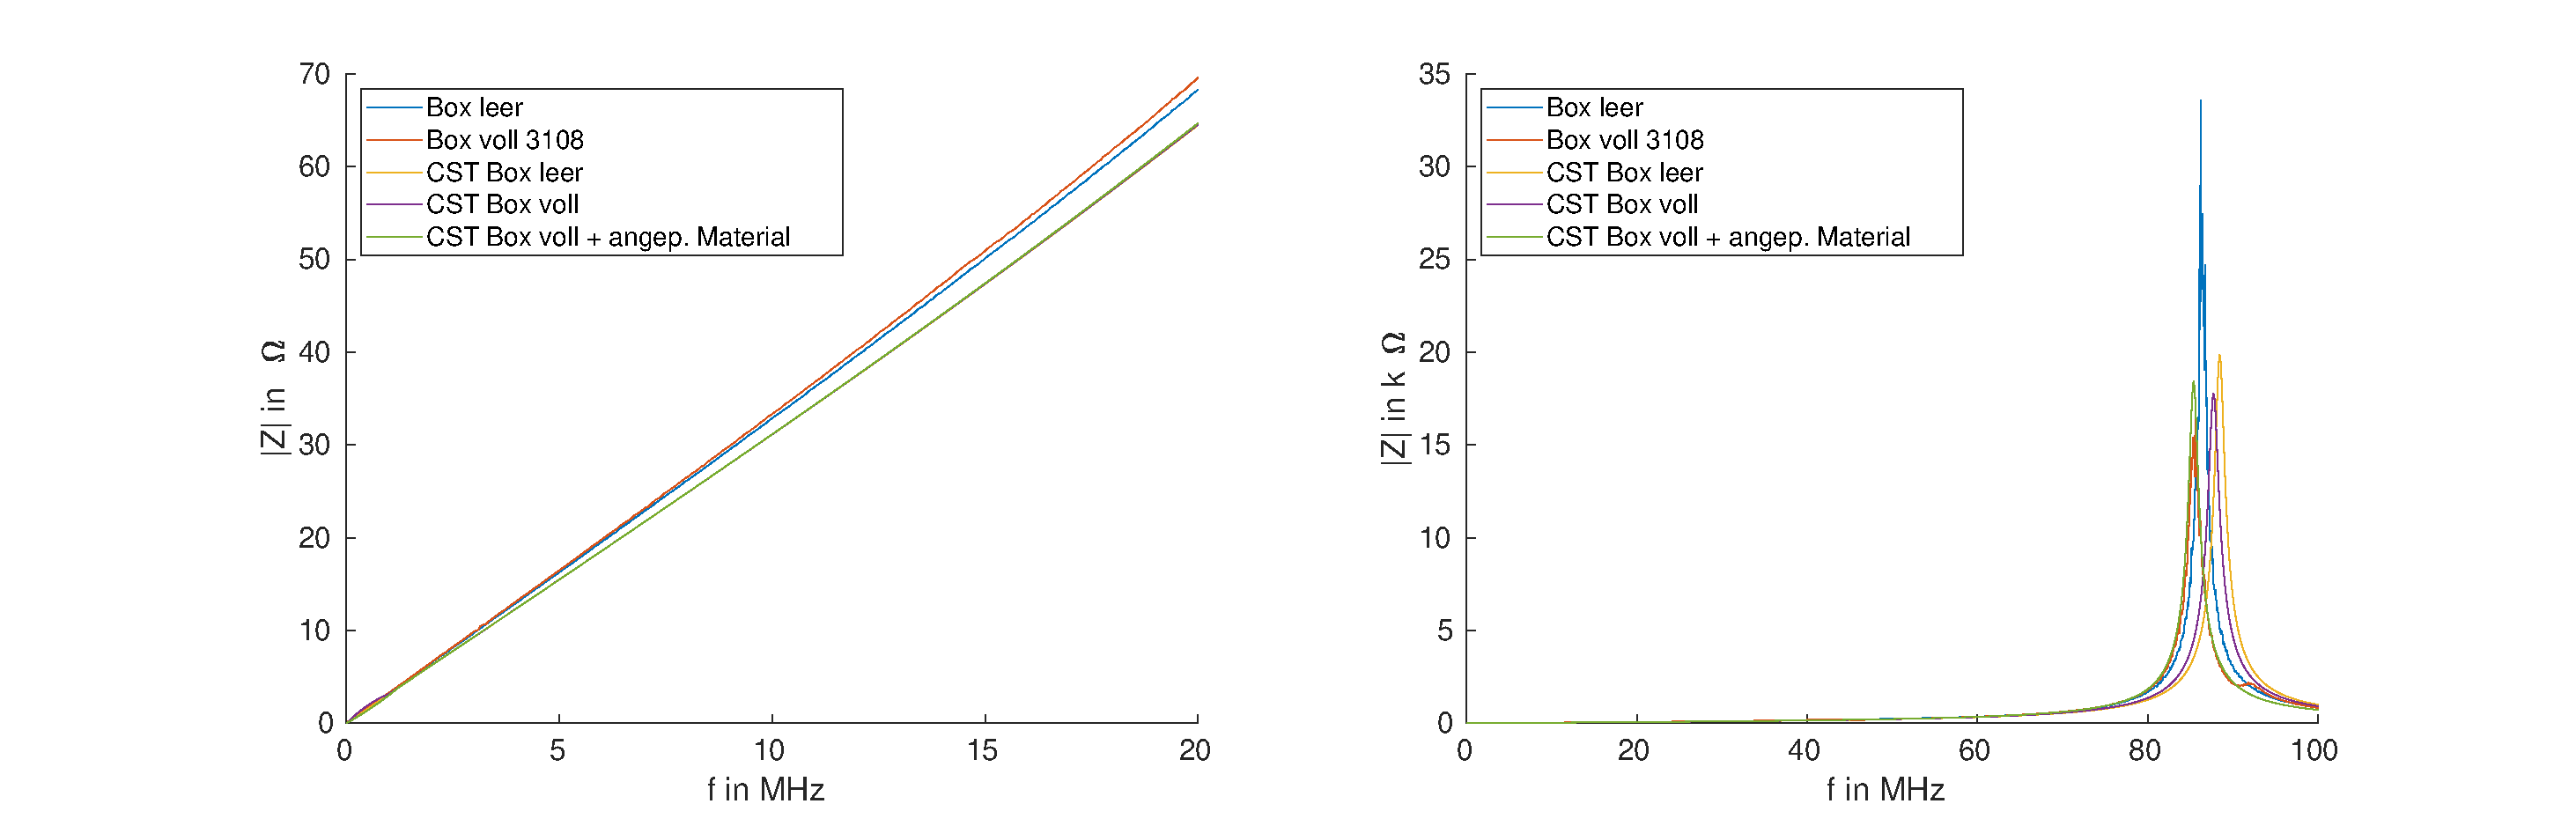
\includegraphics[width=\textwidth]{measurement_simulation_emptybox}
	\caption{Gegen\"uberstellung der Simulation und Messung f\"ur eine Anordnung ohne Ringkern.}
	\label{fig:boxpolycrossrkappend}
\end{figure}

\begin{figure}[htb]
	\centering
	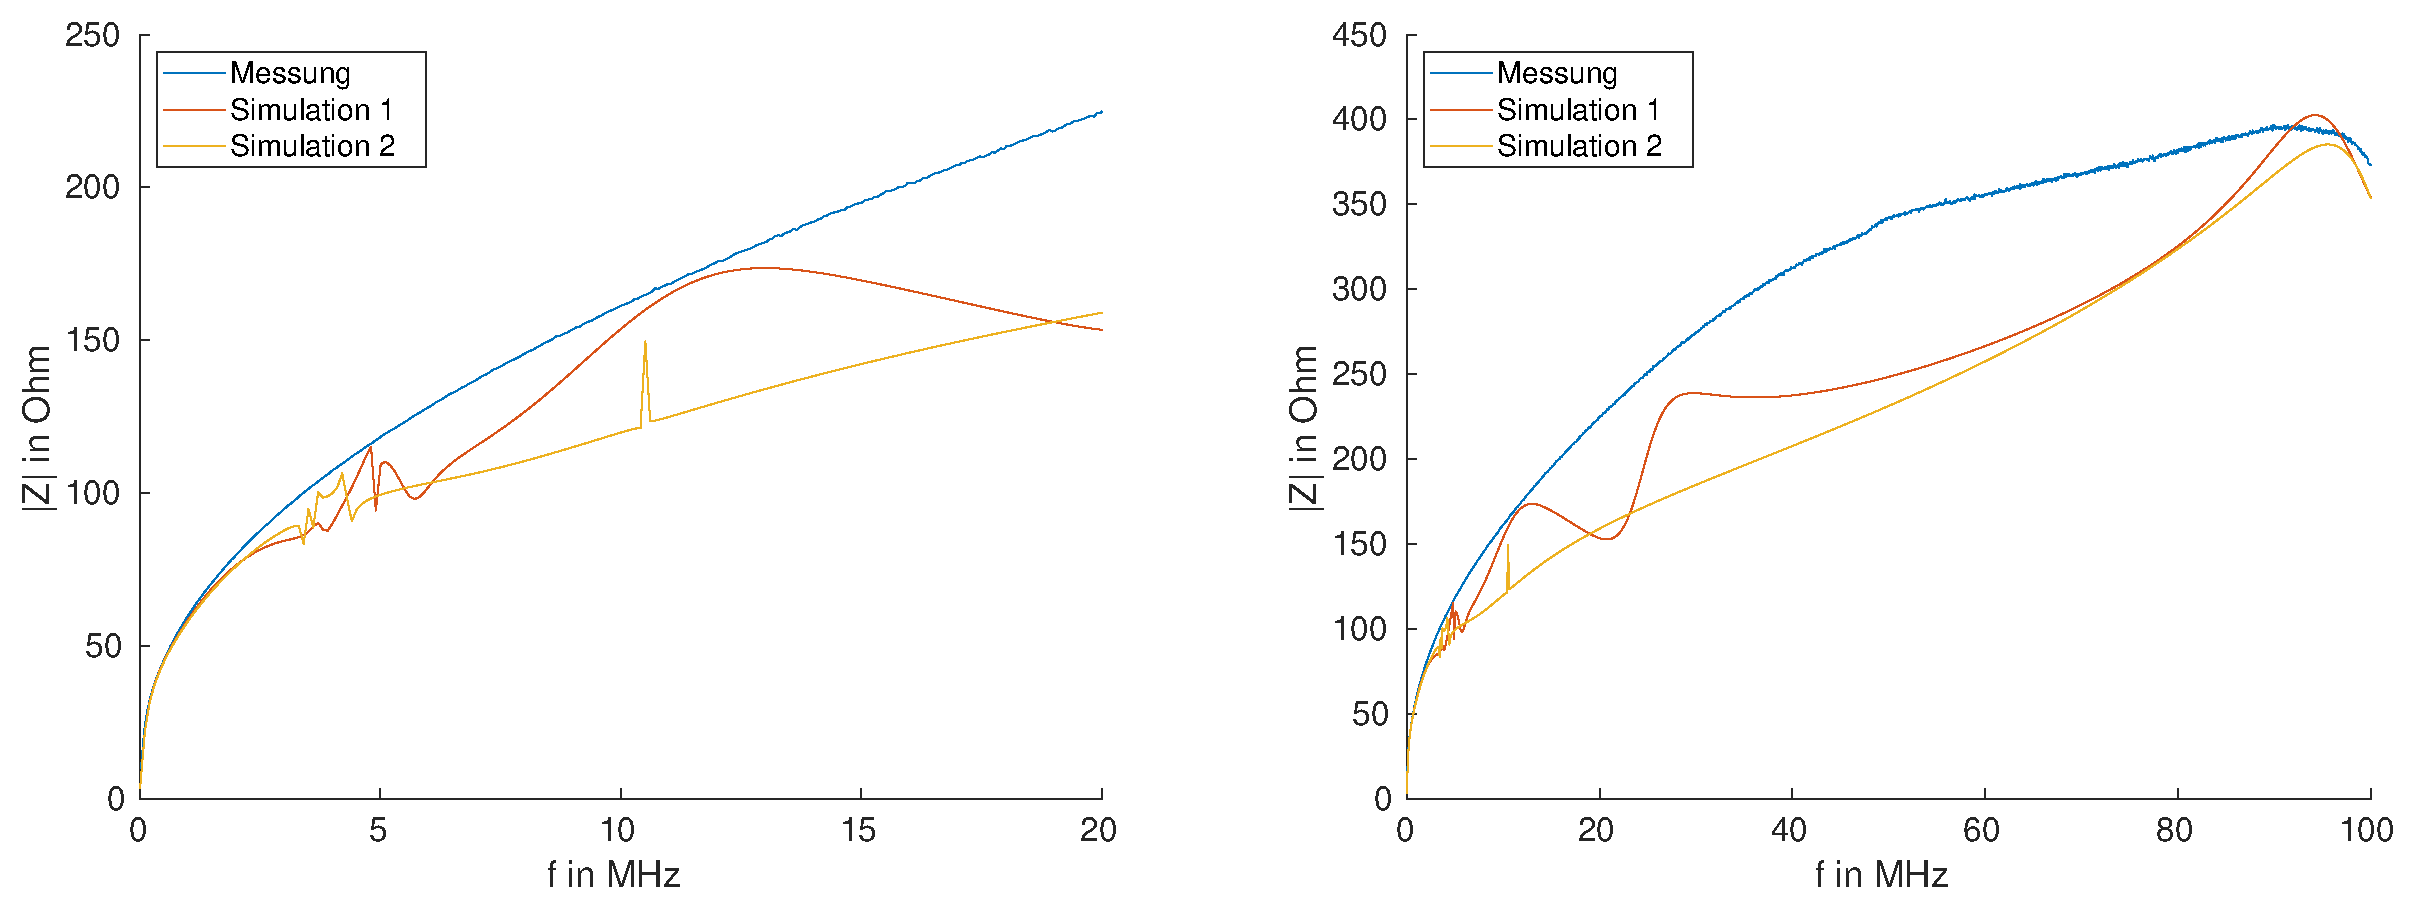
\includegraphics[width=\textwidth]{RK_Impedanz_vergleich}
	\caption{Gegen\"uberstellung der Simulation und Messung f\"ur eine Anordnung mit Ringkern ohne Kurzschl\"usse.}
	\label{fig:boxpolycrossrkappend}
\end{figure}

\begin{figure}[htb]
	\centering
	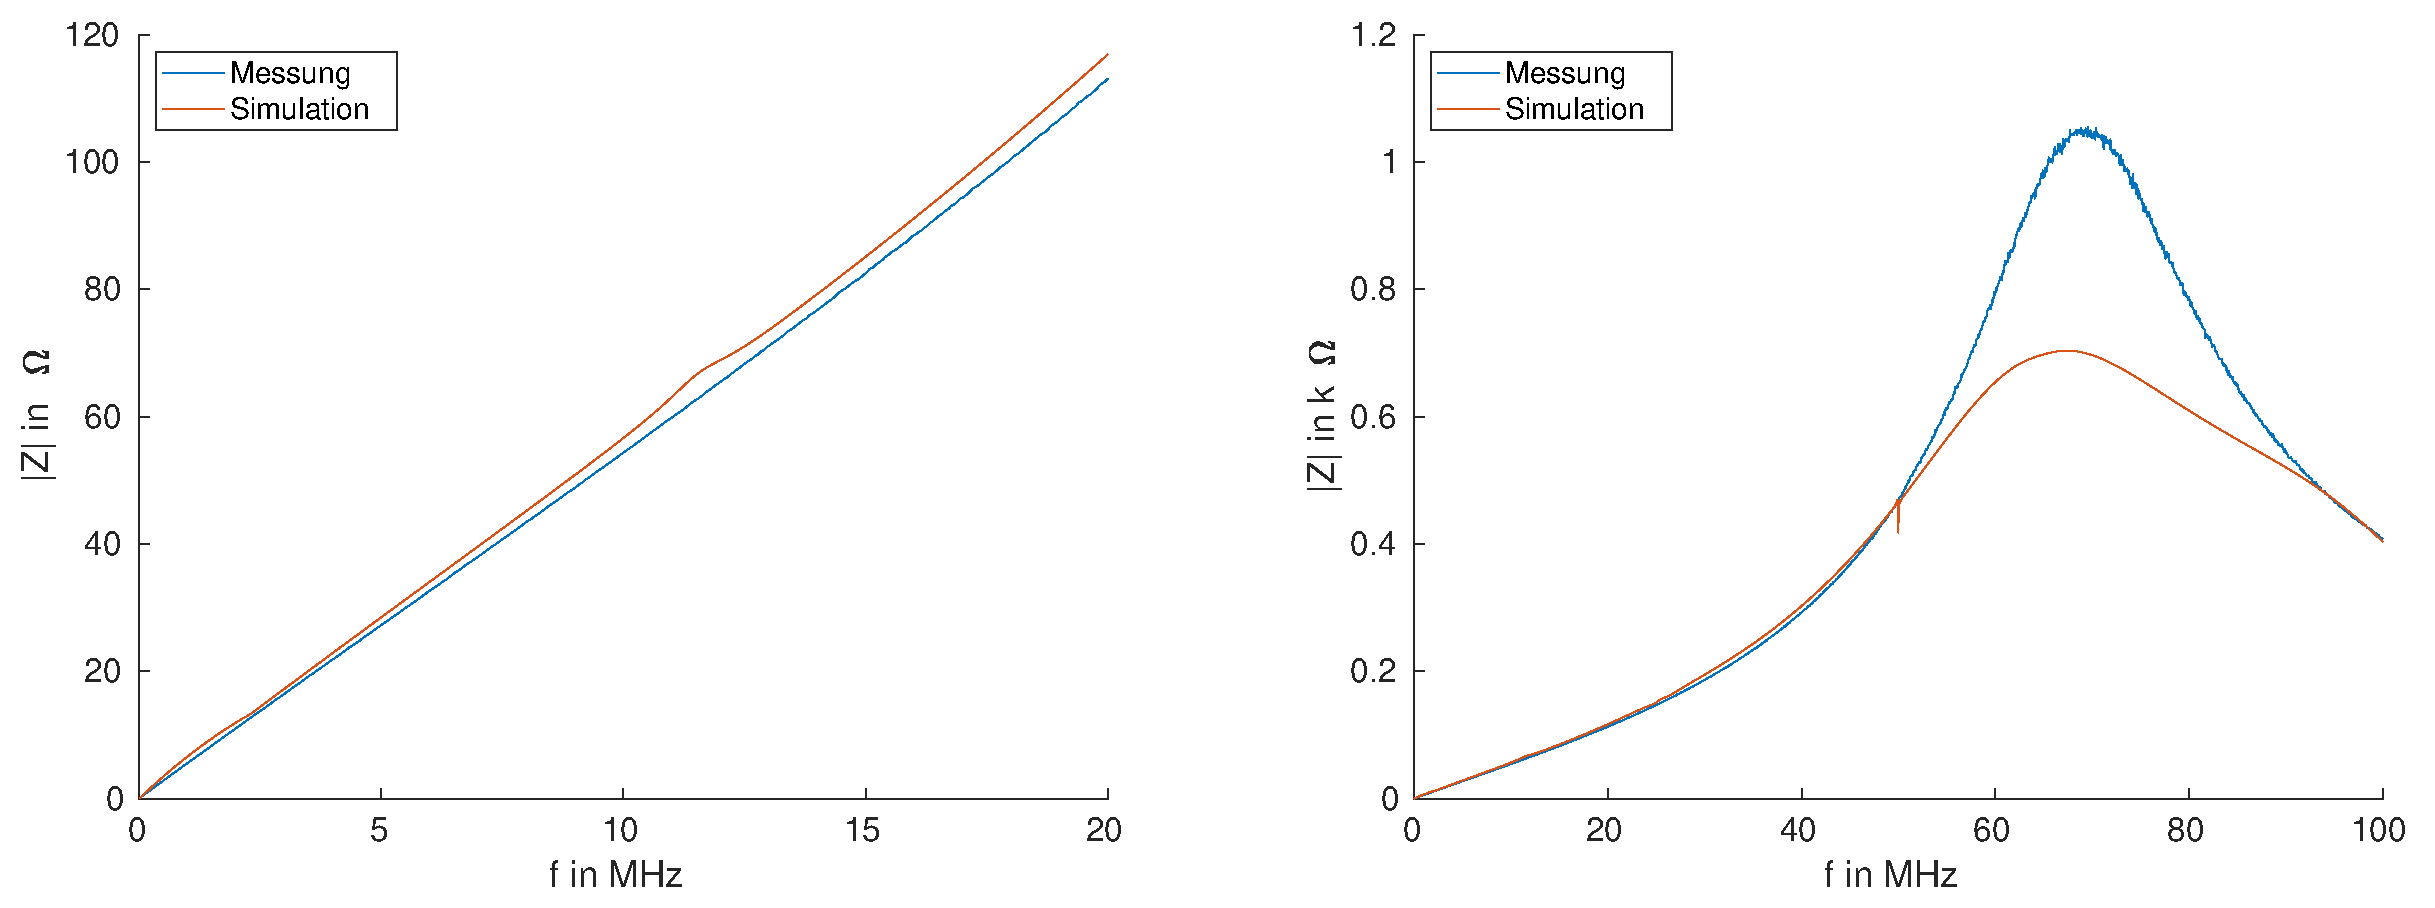
\includegraphics[width=\textwidth]{Z_ges_1KS_SimMeas}
	\caption{Gegen\"uberstellung der Simulation und Messung f\"ur eine Anordnung mit Ringkern mit einem Kurzschluss.}
	\label{fig:boxpolycrossrk1ksappend}
\end{figure}

\begin{figure}[htb]
	\centering
	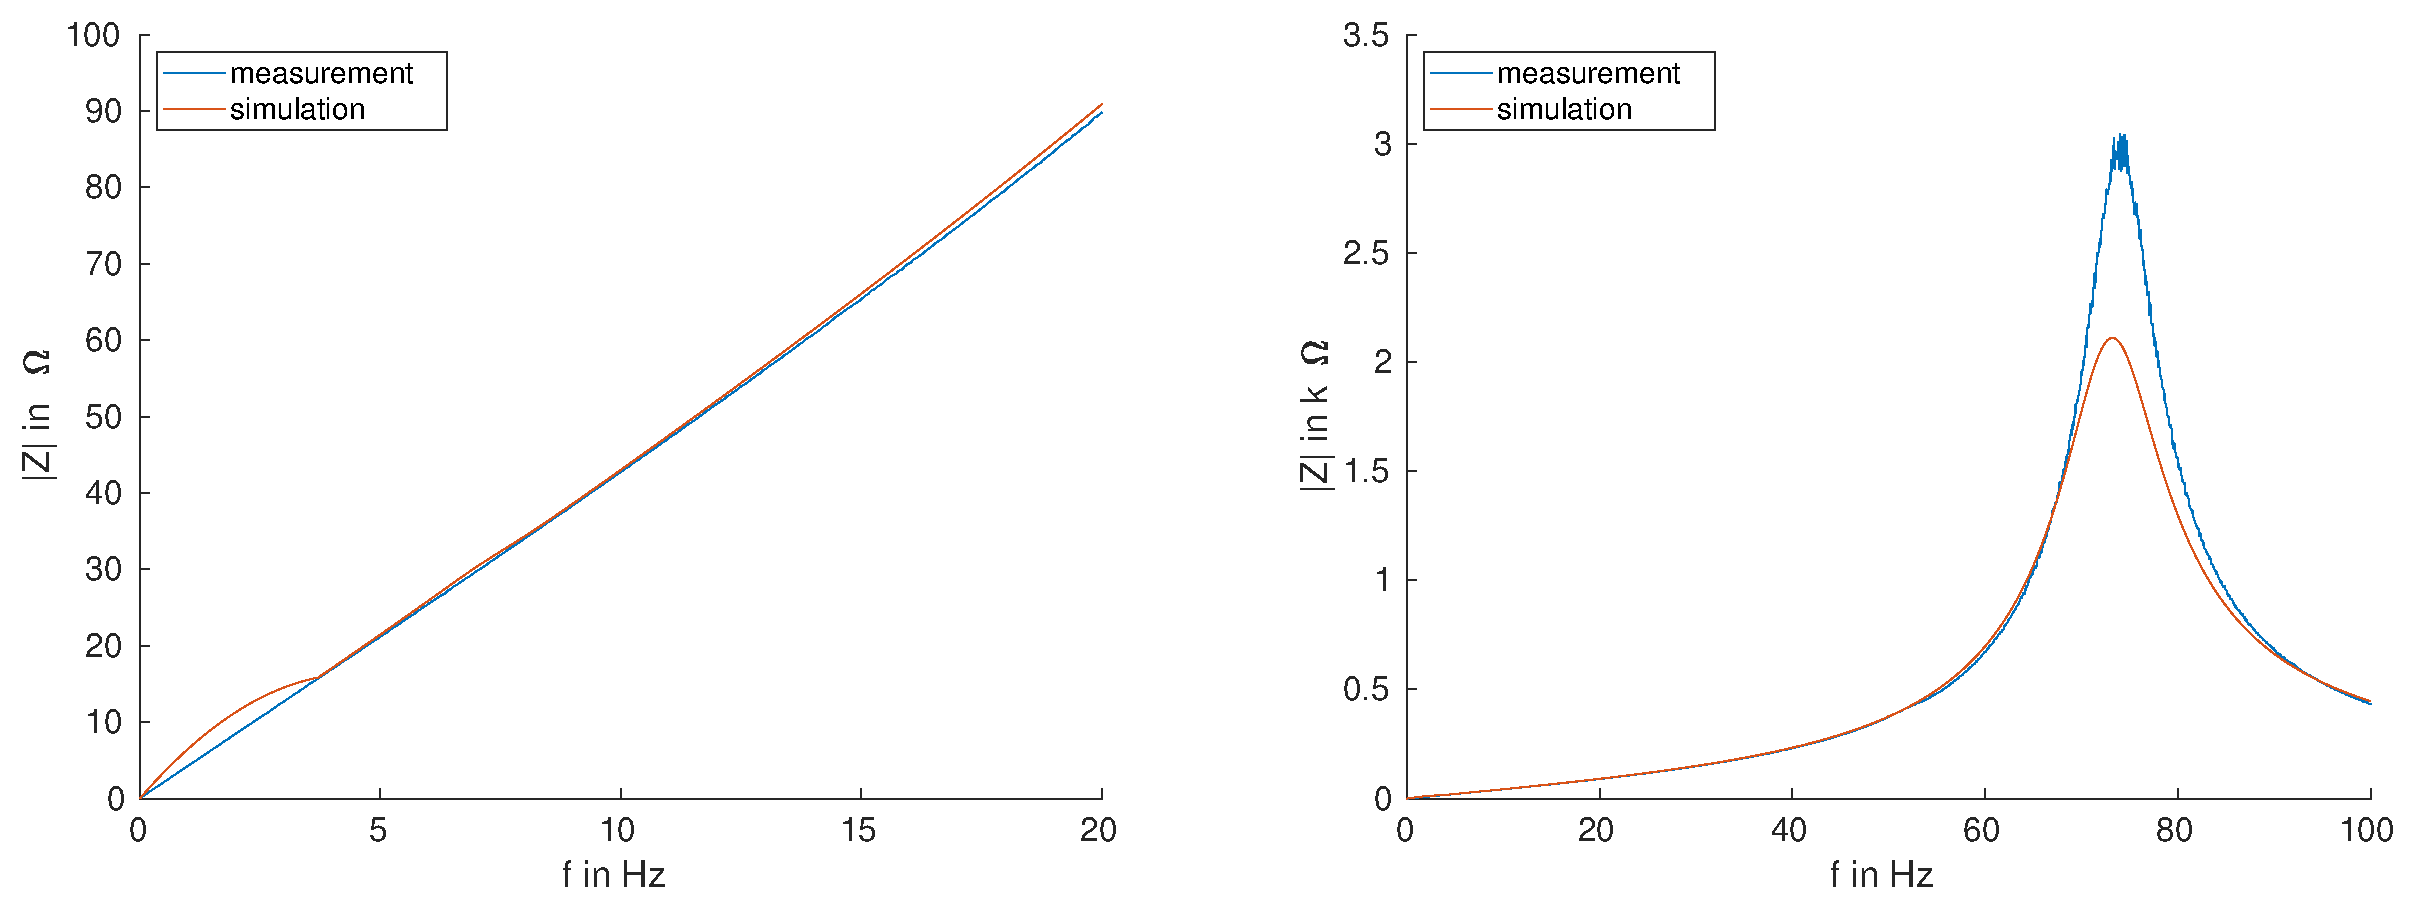
\includegraphics[width=\textwidth]{Z_ges_2KS_SimMeas}
	\caption{Gegen\"uberstellung der Simulation und Messung f\"ur eine Anordnung mit Ringkern mit zwei Kurzschl\"ussen.}
	\label{fig:boxpolycrossrk2ksappend}
\end{figure}

\begin{figure}[htb]
	\centering
	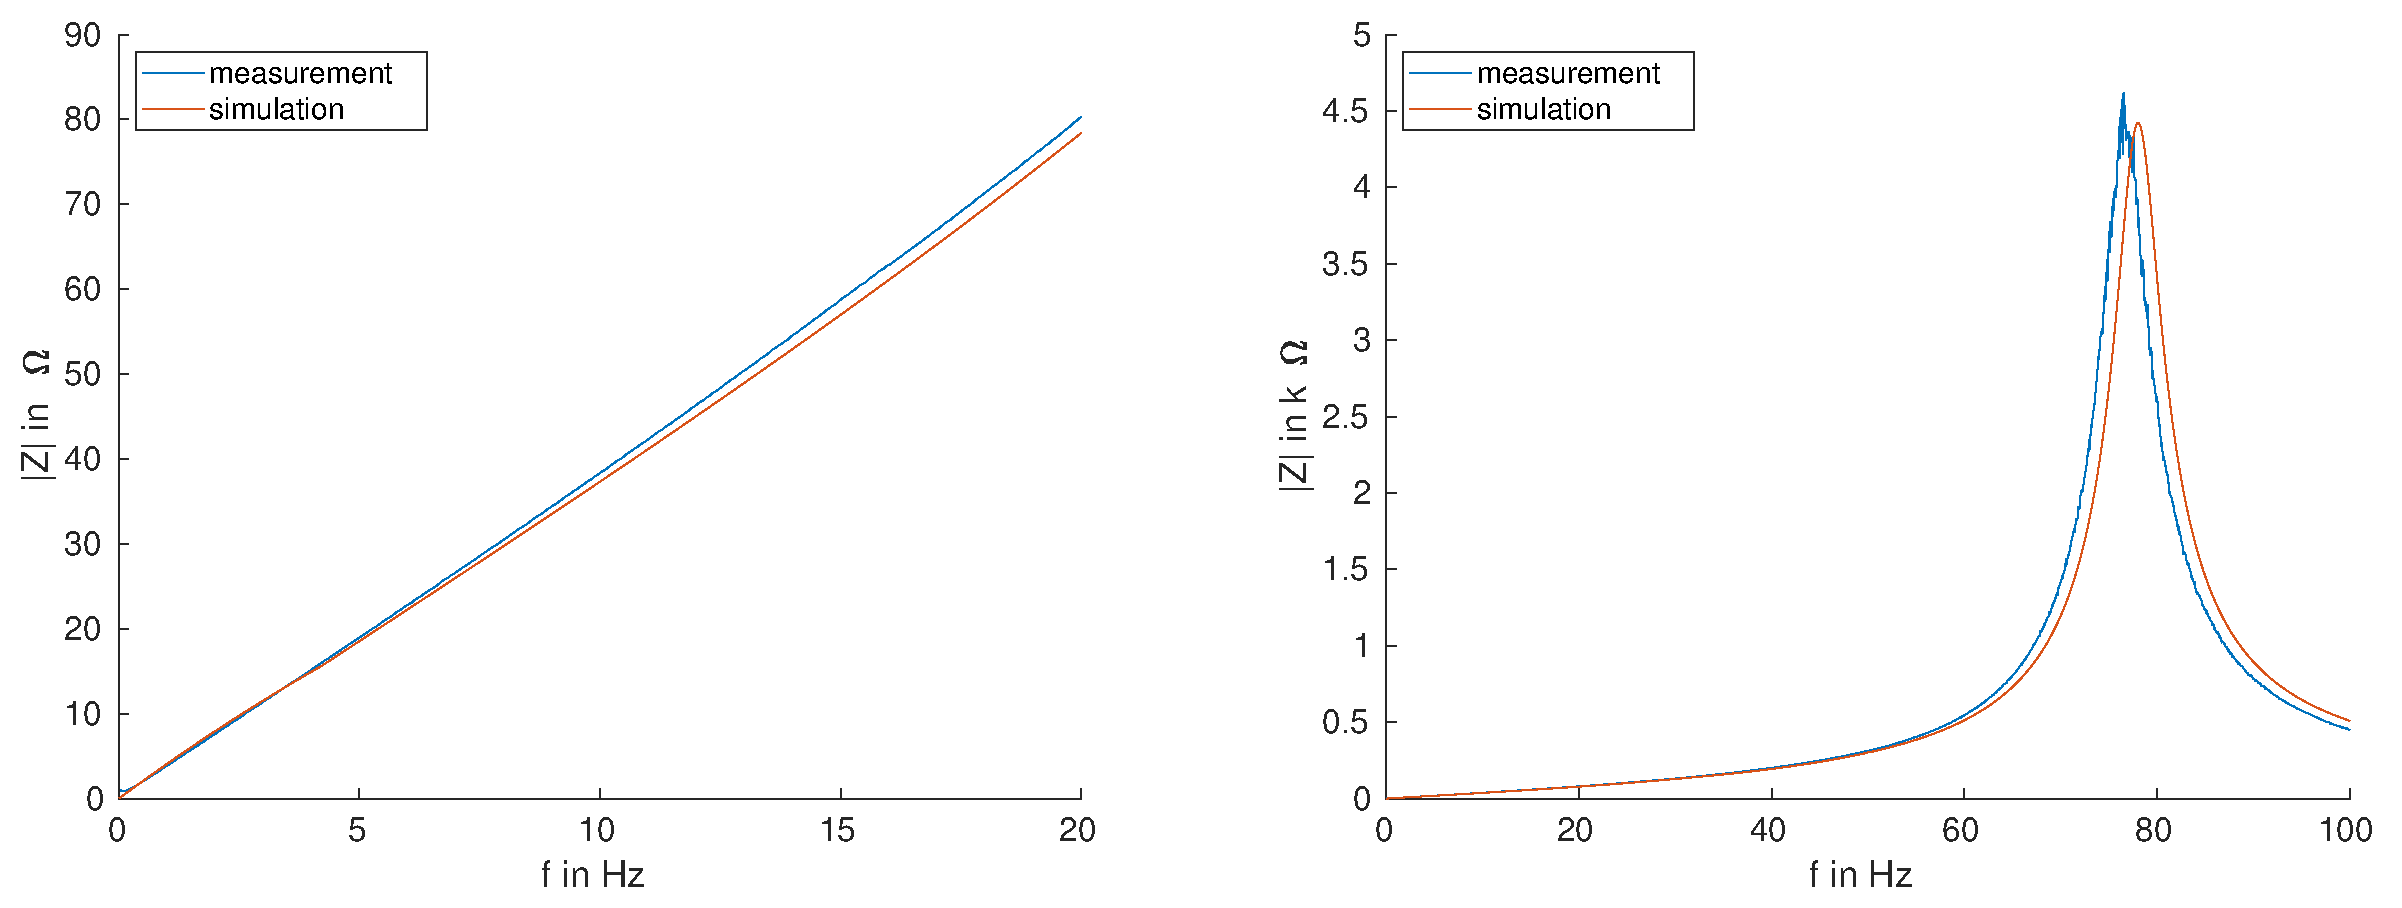
\includegraphics[width=\textwidth]{Z_ges_3KS_SimMeas}
	\caption{Gegen\"uberstellung der Simulation und Messung f\"ur eine Anordnung mit Ringkern mit drei Kurzschl\"ussen.}
	\label{fig:boxpolycrossrk3ksappend}
\end{figure}

\begin{figure}[htb]
	\centering
	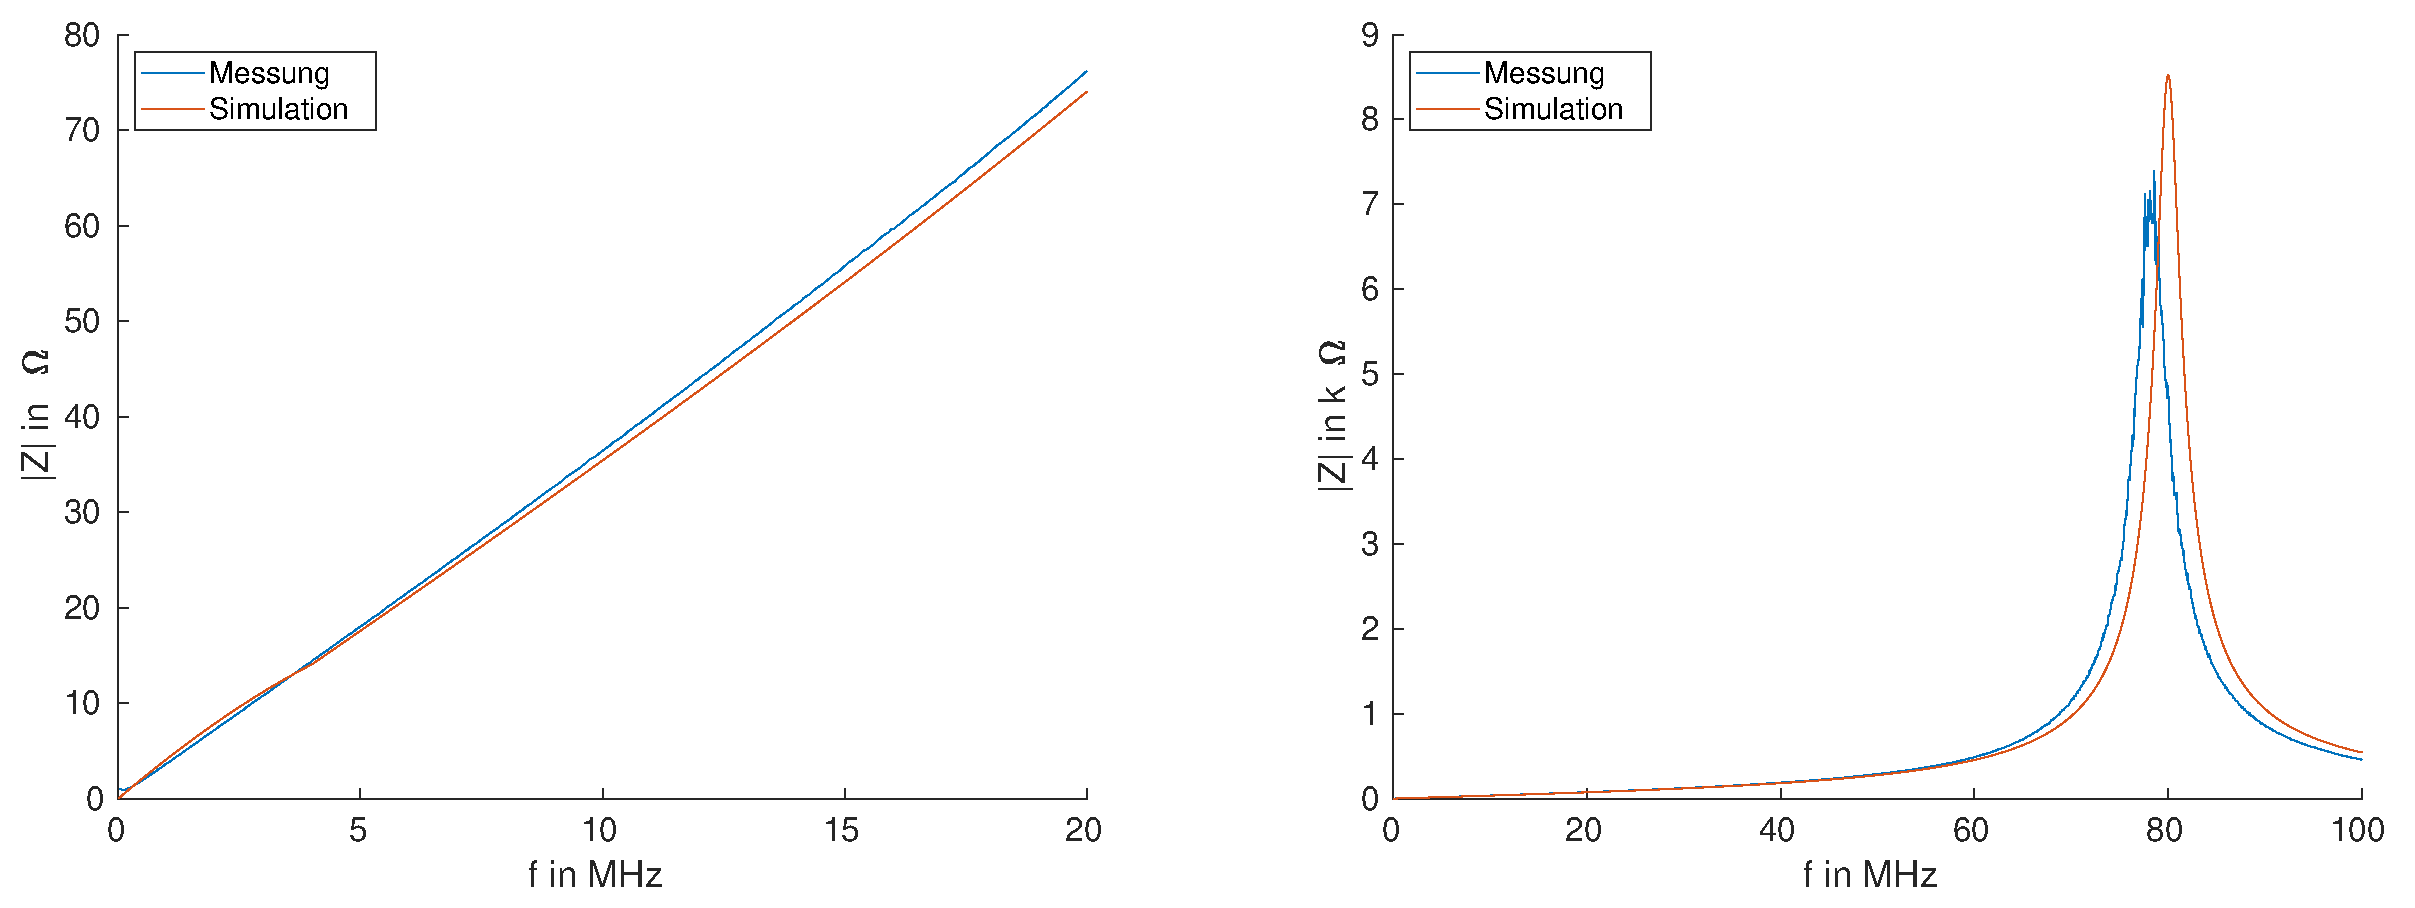
\includegraphics[width=\textwidth]{Z_ges_4KS_SimMeas}
	\caption{Gegen\"uberstellung der Simulation und Messung f\"ur eine Anordnung mit Ringkern mit vier Kurzschl\"ussen.}
	\label{fig:boxpolycrossrk4ksappend}
\end{figure}

\begin{figure}[htb]
	\centering
	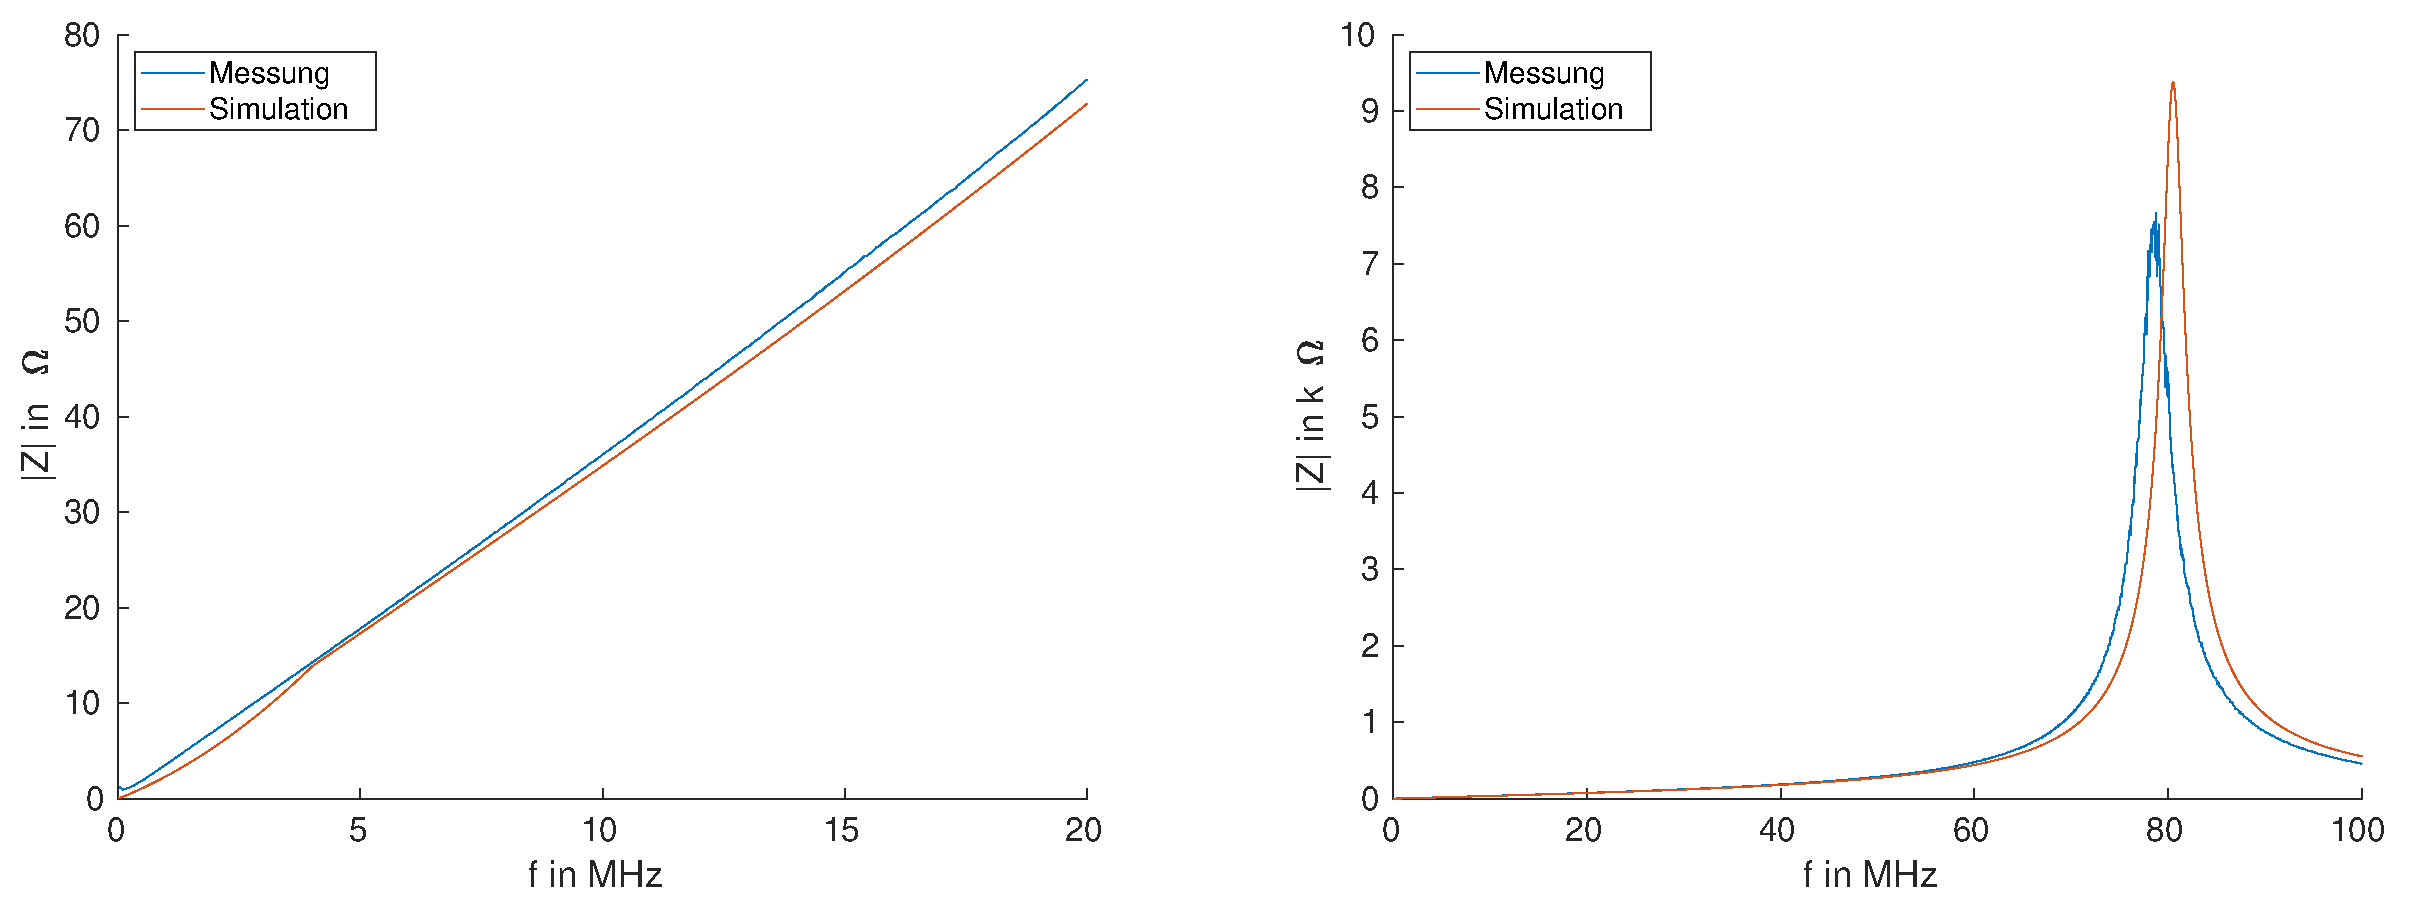
\includegraphics[width=\textwidth]{Z_ges_5KS_SimMeas}
	\caption{Gegen\"uberstellung der Simulation und Messung f\"ur eine Anordnung mit Ringkern mit f\"unf Kurzschl\"ussen.}
	\label{fig:boxpolycrossrk5ksappend}
\end{figure}

\begin{figure}[htb]
	\centering
	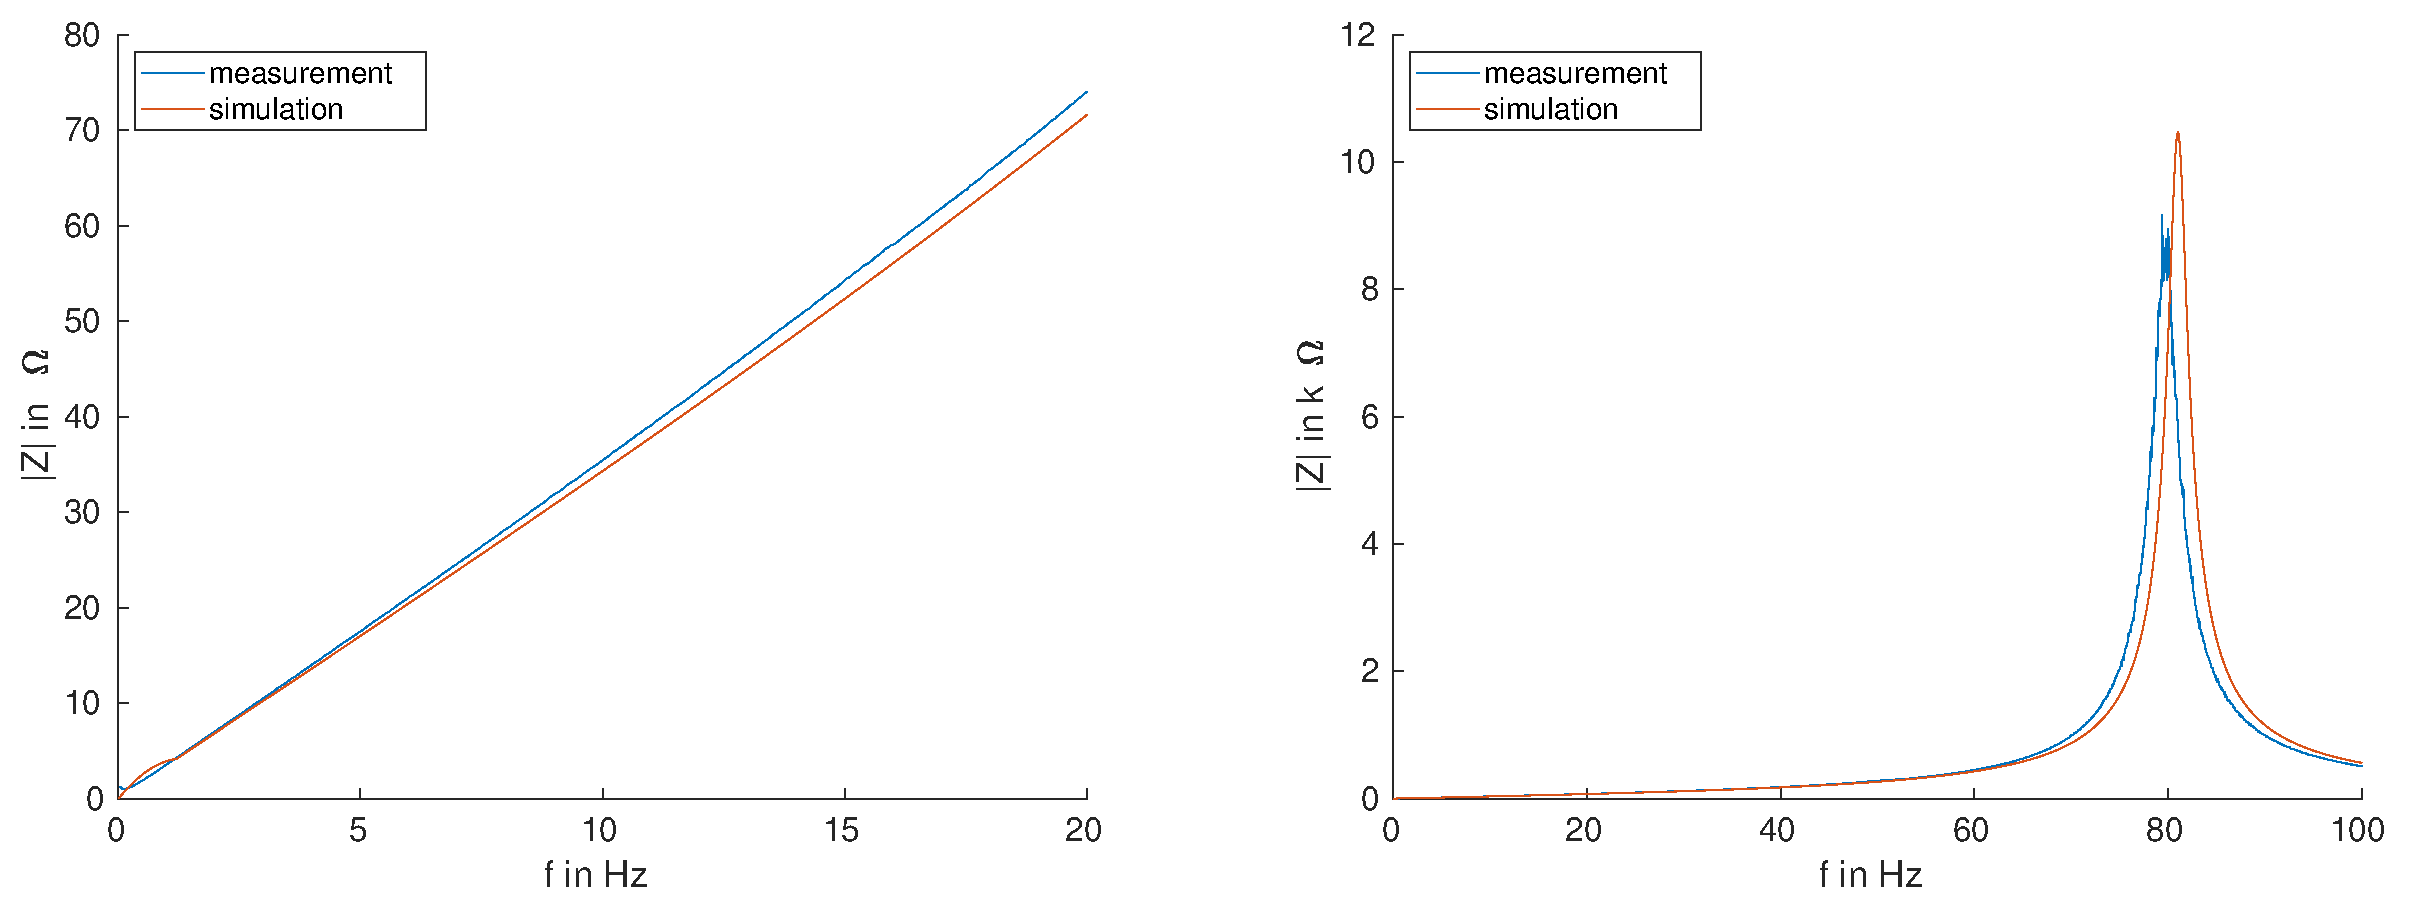
\includegraphics[width=\textwidth]{Z_ges_6KS_SimMeas}
	\caption{Gegen\"uberstellung der Simulation und Messung f\"ur eine Anordnung mit Ringkern mit sechs Kurzschl\"ussen.}
	\label{fig:boxpolycrossrk6ksappend}
\end{figure}

\begin{figure}[htb]
	\centering
	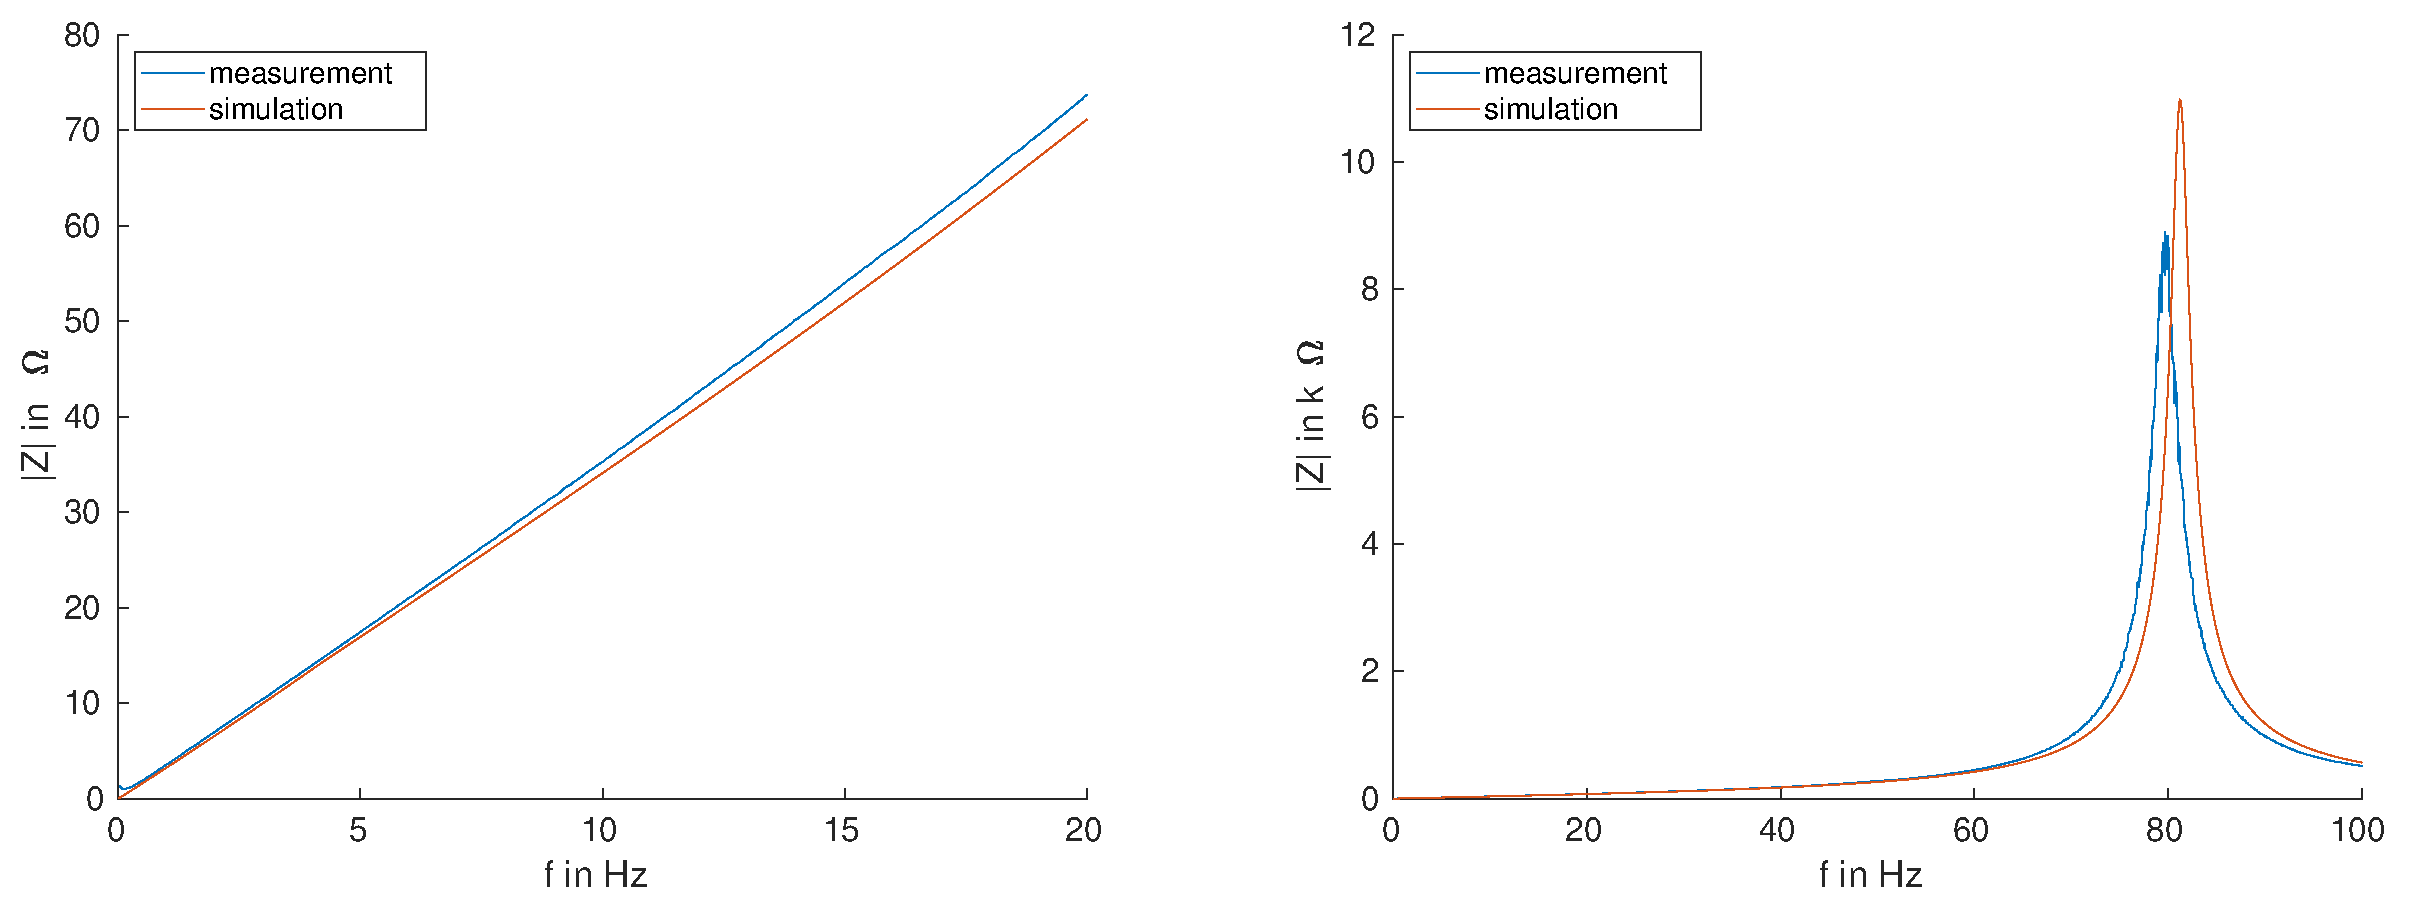
\includegraphics[width=\textwidth]{Z_ges_7KS_SimMeas}
	\caption{Gegen\"uberstellung der Simulation und Messung f\"ur eine Anordnung mit Ringkern mit sieben Kurzschl\"ussen.}
	\label{fig:boxpolycrossrk7ksappend}
\end{figure}

\begin{figure}[htb]
	\centering
	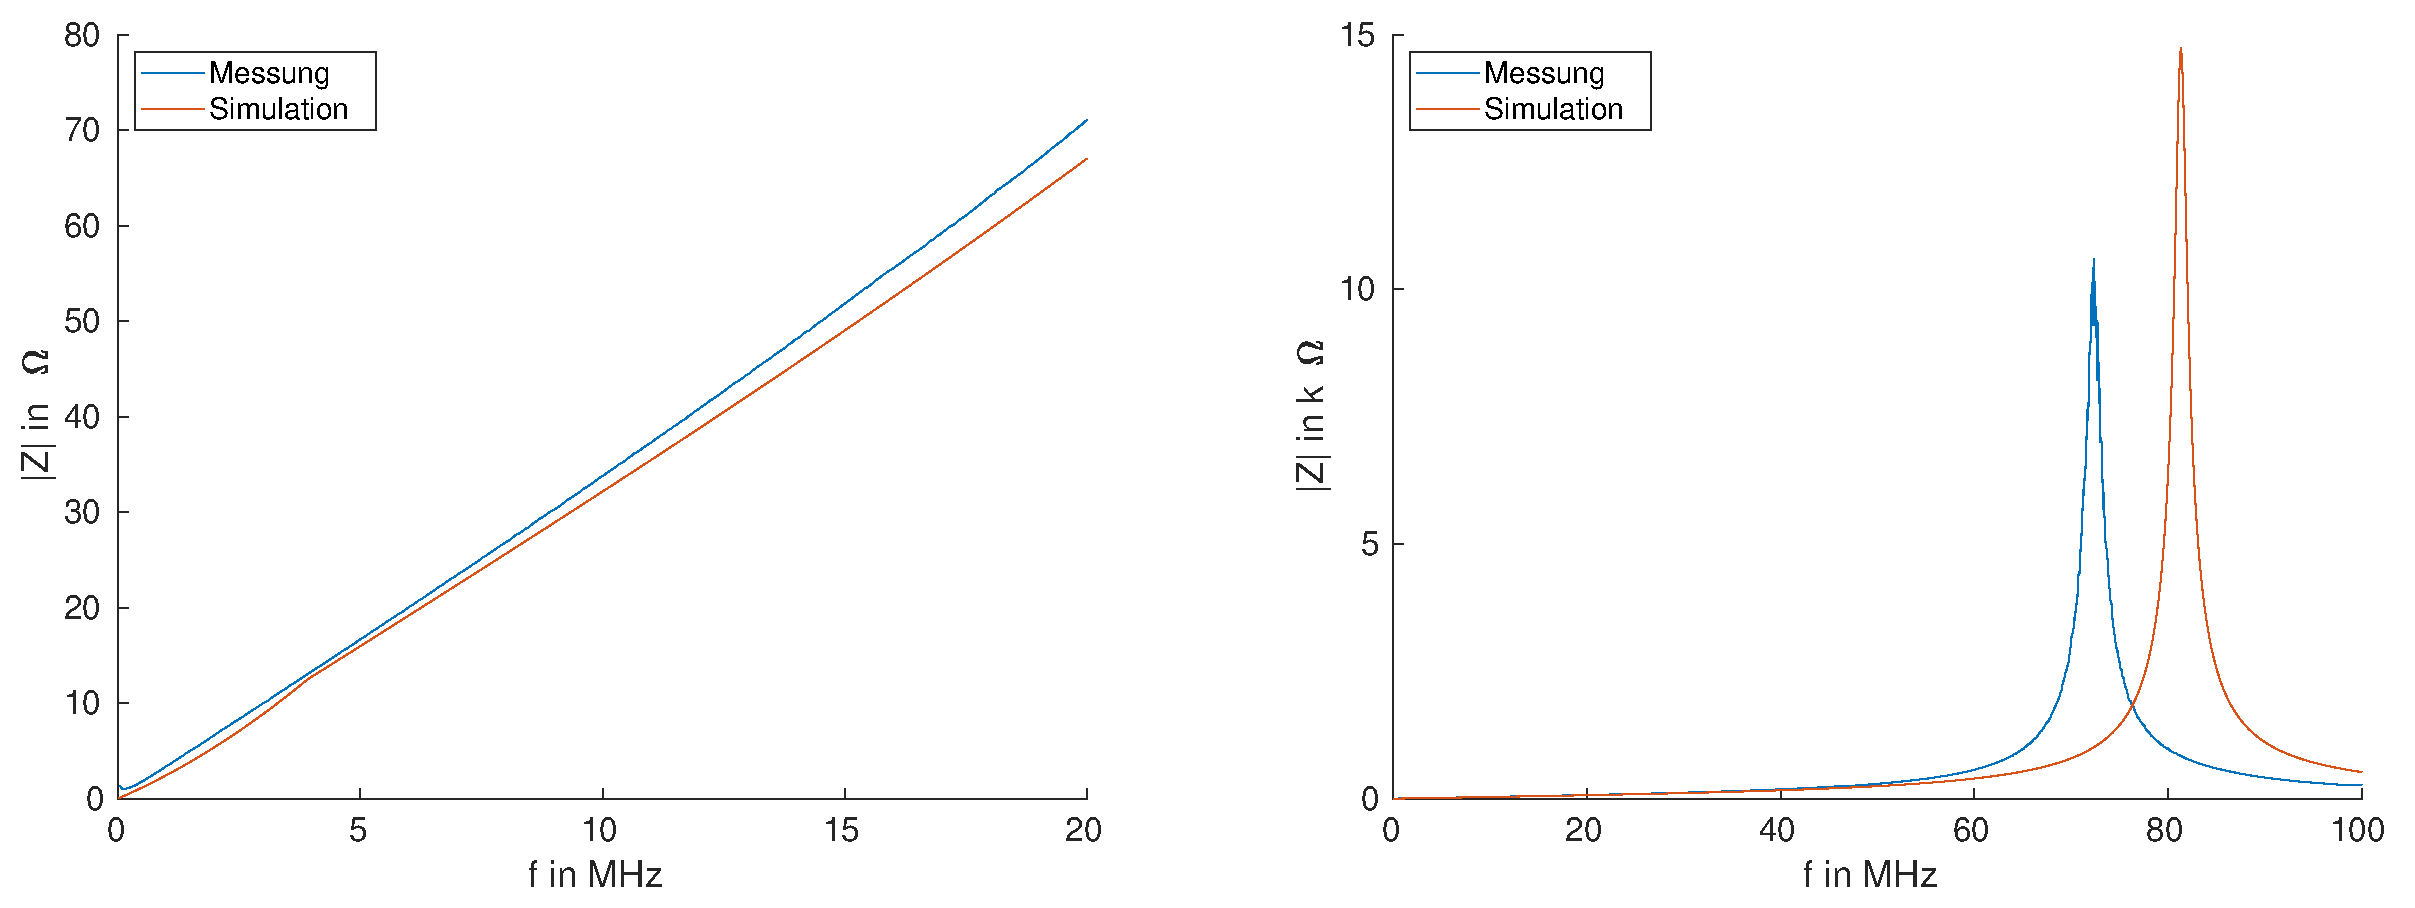
\includegraphics[width=\textwidth]{Z_ges_8KS_SimMeas}
	\caption{Gegen\"uberstellung der Simulation und Messung f\"ur eine Anordnung mit Ringkern mit acht Kurzschl\"ussen.}
	\label{fig:boxpolycrossrk8ksappend}
\end{figure}